\documentclass[11pt,a4paper]{article}

% ---------------------------------------------------------------- packages
\usepackage[T1]{fontenc}
\usepackage[utf8]{inputenc}
\usepackage{lmodern}
\usepackage[margin=2.3cm]{geometry}
\usepackage{graphicx}
\usepackage{booktabs}
\usepackage{tabularx}
\usepackage{multirow}
\usepackage{array}
\usepackage{amsmath}
\usepackage{xcolor}
\usepackage{caption}
\usepackage{subcaption}
\usepackage{float}
\usepackage{enumitem}
\usepackage{listings}
\usepackage{tikz}
\usetikzlibrary{arrows.meta,positioning,fit,backgrounds,shapes.geometric,calc}
\usepackage[hidelinks]{hyperref}

\graphicspath{{../outputs/figures/}{../outputs/results/val/}{../train/runs/}}
\setlist{itemsep=2pt,topsep=4pt}
\captionsetup{font=small,labelfont=bf}

\definecolor{seriesA}{HTML}{2A78D6}
\definecolor{seriesB}{HTML}{EB6834}
\definecolor{stageData}{HTML}{E8F1FB}
\definecolor{stageProc}{HTML}{FDEDE6}
\definecolor{stageEval}{HTML}{E5F6EF}
\definecolor{ink}{HTML}{0B0B0B}
\definecolor{ink2}{HTML}{52514E}

\lstset{basicstyle=\ttfamily\footnotesize,columns=fullflexible,breaklines=true,frame=single,
        framerule=0.3pt,rulecolor=\color{ink2!40},backgroundcolor=\color{black!2}}

\newcommand{\code}[1]{\texttt{\small #1}}

% ---------------------------------------------------------------- title
\title{\textbf{Synthetic Deformable Waste Data Generation\\for Sim-to-Real Perception}\\[6pt]
\large AI512 -- Project 2: Project Report}

\author{
\begin{tabular}{c}
\rule{6cm}{0.4pt}\\[-2pt]
\small Author 1 \\[4pt]
\small Entry No.: \rule{3.5cm}{0.4pt}
\end{tabular}
\quad
\begin{tabular}{c}
\rule{6cm}{0.4pt}\\[-2pt]
\small Author 2 \\[4pt]
\small Entry No.: \rule{3.5cm}{0.4pt}
\end{tabular}
\\[18pt]
\begin{tabular}{c}
\rule{6cm}{0.4pt}\\[-2pt]
\small Author 3 \\[4pt]
\small Entry No.: \rule{3.5cm}{0.4pt}
\end{tabular}
}
\date{November 2026}

\begin{document}
\maketitle

% ================================================================ abstract
\begin{abstract}
Waste-sorting robots and litter-detection systems must recognise packaging that is crushed,
dented or bent, yet labelled real images of deformed waste are scarce and 3D asset libraries
contain almost exclusively intact objects. We present a reproducible pipeline that generates
labelled synthetic training data of \emph{deformable} waste. Intact 3D models of four classes
(bottle, can, cup, carton) are taken from Objaverse, normalised to real-world scale and
procedurally deformed in Blender (crush and bend, each at three severity levels, deterministic
from a seed). Domain-randomised scenes are rendered with BlenderProc, yielding pixel-accurate
COCO masks, YOLO boxes and per-object deformation metadata. In a controlled experiment we train
two YOLO11n detectors on 1200 identical scenes that differ only in whether objects are deformed
(A: intact only; B: $\approx$60\,\% deformed) and evaluate them on synthetic test scenes and on
1500 real litter photographs from TACO. Training with deformations raises mAP50 on deformed
synthetic objects from 0.889 to 0.936 and recall on medium-crushed objects from 0.66 to 0.93,
at a cost of only 0.012 mAP50 on intact objects. On real TACO photos model B outperforms model A
overall (mAP50 0.051 vs.\ 0.042) and for every class, but absolute scores remain low, showing
that the appearance gap between clean renders and real litter dominates the sim-to-real
transfer.
\end{abstract}

\tableofcontents
\newpage

% ================================================================ introduction
\section{Introduction}

Automated waste sorting and litter monitoring rely on object detectors that localise and
classify items such as bottles, cans, cups and cartons in camera images. In practice, discarded
packaging is rarely in pristine condition: cans are stepped on, bottles are squeezed and cartons
are folded. Detectors trained on images of intact objects therefore face a distribution shift
in the very situations they are deployed in.

Collecting and annotating large numbers of real photographs of deformed waste is slow and
expensive. Synthetic data generation offers an alternative: objects are rendered in randomised
virtual scenes and the renderer provides exact annotations at no cost. However, publicly
available 3D model collections such as Objaverse~\cite{objaverse} contain almost only intact,
undamaged products, so standard synthetic pipelines inherit the same bias.

\paragraph{Research question.} \emph{Does adding procedurally deformed objects to synthetic
training data improve the detection of real-world deformed waste, compared with training on
intact objects only?}

\paragraph{Contributions.}
\begin{enumerate}
  \item A configurable, one-command pipeline that downloads and normalises CC-licensed 3D models,
        deforms them procedurally at controlled severity levels, renders domain-randomised
        scenes and produces COCO and YOLO annotations with deformation metadata.
  \item Two matched synthetic datasets (1200 images each, 4 classes): \emph{A\_intact} and
        \emph{B\_deformed}, generated from identical per-scene seeds so that deformation is the
        only difference.
  \item A controlled detection experiment with YOLO11n~\cite{yolo11}, evaluated on synthetic test
        scenes (broken down by deformation type and level) and on the real TACO
        dataset~\cite{taco}.
\end{enumerate}

% ================================================================ related work
\section{Background and Related Work}

\textbf{Domain randomisation.} Tobin et al.~\cite{tobin} showed that randomising textures,
lighting and camera poses in simulation lets networks trained purely on synthetic images
transfer to the real world, by making reality appear as ``just another variation''. Tremblay
et al.~\cite{tremblay} extended this to object detection with random distractor objects and
showed competitive performance compared with real-data training.

\textbf{Synthetic data tools.} BlenderProc~\cite{blenderproc} is a procedural rendering pipeline
built on Blender that provides physics-based object placement, photorealistic path tracing and
writers for segmentation and COCO annotations. We use it for scene generation.

\textbf{3D assets.} Objaverse~\cite{objaverse} provides around 800k 3D models with per-object
licences; a subset of about 47k models carries LVIS category labels, which we use to locate
bottles, cans, cups and cartons.

\textbf{Litter datasets.} TACO~\cite{taco} contains 1500 photographs of litter in natural
environments with 60 fine-grained categories, many of them crushed or dirty. We use it
exclusively as a real-world test set.

% ================================================================ method
\section{Method}

\subsection{Pipeline overview}

Figure~\ref{fig:pipeline} shows the complete workflow. Every stage is a stand-alone script in
\code{src/} that reads the central configuration file \code{configs/pipeline.yaml}; the
orchestrator \code{run\_pipeline.py} runs the stages in order and logs each one.

\begin{figure}[H]
\centering
\resizebox{\textwidth}{!}{%
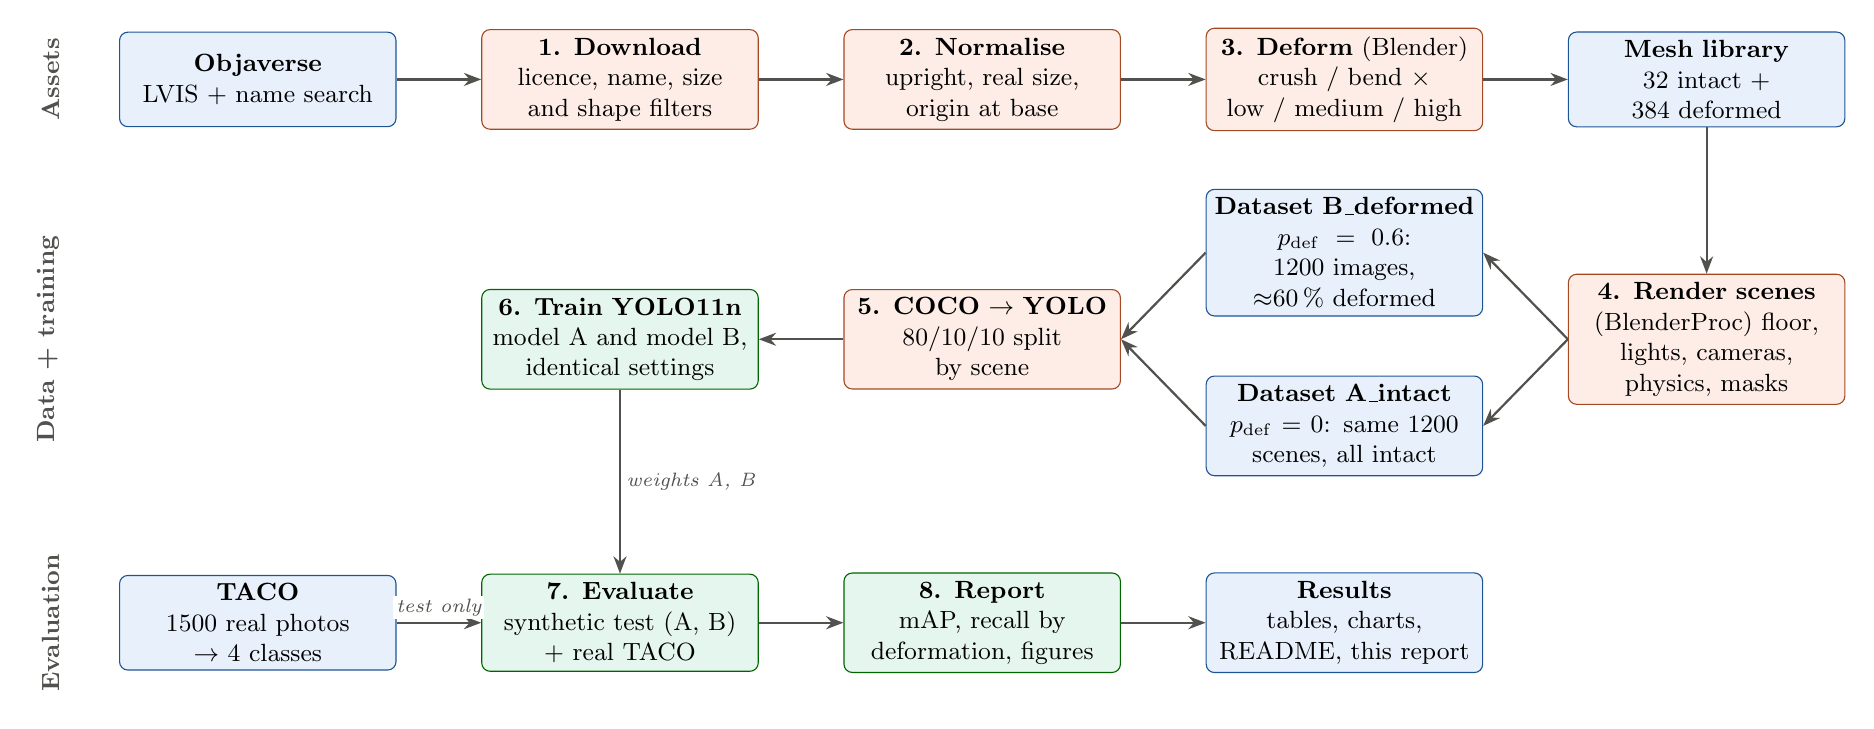
\begin{tikzpicture}[
  every node/.style={font=\small},
  base/.style={rounded corners=3pt, align=center, minimum height=12mm, text width=33mm, inner sep=3pt},
  data/.style={base, draw=seriesA!70!black, fill=stageData},
  proc/.style={base, draw=seriesB!70!black, fill=stageProc},
  evalb/.style={base, draw=green!40!black, fill=stageEval},
  arr/.style={-{Stealth[length=2.2mm]}, thick, color=ink2},
  lab/.style={font=\scriptsize\itshape, color=ink2, fill=white, inner sep=1pt},
  row/.style={font=\small\bfseries, color=ink2, rotate=90, anchor=south}
]
\def\dx{4.6}
% ---------------- row 1: asset generation (left to right)
\node[data]  (obj)    at (0*\dx, 0)  {\textbf{Objaverse}\\LVIS + name search};
\node[proc]  (dl)     at (1*\dx, 0)  {\textbf{1. Download}\\licence, name, size\\and shape filters};
\node[proc]  (norm)   at (2*\dx, 0)  {\textbf{2. Normalise}\\upright, real size,\\origin at base};
\node[proc]  (def)    at (3*\dx, 0)  {\textbf{3. Deform} (Blender)\\crush / bend $\times$\\low / medium / high};
\node[data]  (mesh)   at (4*\dx, 0)  {\textbf{Mesh library}\\32 intact +\\384 deformed};
\draw[arr] (obj) -- (dl);  \draw[arr] (dl) -- (norm);
\draw[arr] (norm) -- (def); \draw[arr] (def) -- (mesh);

% ---------------- row 2: synthetic data + training (right to left)
\node[proc]  (render) at (4*\dx, -3.3) {\textbf{4. Render scenes}\\(BlenderProc) floor,\\lights, cameras,\\physics, masks};
\node[data]  (dsB)    at (3*\dx, -2.2) {\textbf{Dataset B\_deformed}\\$p_\mathrm{def}=0.6$: 1200 images,\\$\approx$60\,\% deformed};
\node[data]  (dsA)    at (3*\dx, -4.4) {\textbf{Dataset A\_intact}\\$p_\mathrm{def}=0$: same 1200\\scenes, all intact};
\node[proc]  (yolo)   at (2*\dx, -3.3) {\textbf{5. COCO $\rightarrow$ YOLO}\\80/10/10 split\\by scene};
\node[evalb] (train)  at (1*\dx, -3.3) {\textbf{6. Train YOLO11n}\\model A and model B,\\identical settings};
\draw[arr] (mesh) -- (render);
\draw[arr] (render.west) -- (dsB.east);
\draw[arr] (render.west) -- (dsA.east);
\draw[arr] (dsB.west) -- (yolo.east);
\draw[arr] (dsA.west) -- (yolo.east);
\draw[arr] (yolo) -- (train);

% ---------------- row 3: evaluation (left to right)
\node[data]  (taco)   at (0*\dx, -6.9) {\textbf{TACO}\\1500 real photos\\$\rightarrow$ 4 classes};
\node[evalb] (eval)   at (1*\dx, -6.9) {\textbf{7. Evaluate}\\synthetic test (A, B)\\+ real TACO};
\node[evalb] (report) at (2*\dx, -6.9) {\textbf{8. Report}\\mAP, recall by\\deformation, figures};
\node[data]  (out)    at (3*\dx, -6.9) {\textbf{Results}\\tables, charts,\\README, this report};
\draw[arr] (train) -- node[lab, right=1pt] {weights A, B} (eval);
\draw[arr] (taco) -- node[lab, above=1pt] {test only} (eval);
\draw[arr] (eval) -- (report); \draw[arr] (report) -- (out);

% ---------------- row labels
\node[row] at (-2.4, 0)    {Assets};
\node[row] at (-2.4, -3.3) {Data + training};
\node[row] at (-2.4, -6.9) {Evaluation};
\end{tikzpicture}}
\caption{End-to-end workflow. Blue boxes are data, orange boxes are generation stages, green
boxes are learning and evaluation stages. Rendering the same seeded scenes with deformation
probability $p_\mathrm{def}=0.6$ and $p_\mathrm{def}=0$ yields the matched datasets B and A. All
stages are driven by \code{configs/pipeline.yaml} and run with
\code{python run\_pipeline.py -{}-stages all}.}
\label{fig:pipeline}
\end{figure}

\subsection{Classes and asset acquisition}

We consider four common, deformable packaging classes, each mapped to the matching TACO
categories for real-world testing (Table~\ref{tab:classes}).

\begin{table}[H]
\centering
\small
\begin{tabularx}{\textwidth}{c l X X c}
\toprule
ID & Class & Objaverse source & TACO categories (test) & Height \\
\midrule
0 & bottle & LVIS bottle, water/beer/wine\_bottle & Clear plastic bottle, Glass bottle, Other plastic bottle & 25\,cm \\
1 & can & LVIS can, beer\_can & Drink can, Food Can & 12\,cm \\
2 & cup & LVIS cup, Dixie\_cup + name search & Disposable plastic cup, Foam cup, Paper cup, Other plastic cup & 10\,cm \\
3 & carton & LVIS carton + name search & Drink carton, Other carton & 20\,cm \\
\bottomrule
\end{tabularx}
\caption{Detection classes, 3D model sources, TACO mapping and normalised real-world height.}
\label{tab:classes}
\end{table}

Candidates are collected from the LVIS-annotated subset of Objaverse and, for cups and cartons
where LVIS is sparse, from a keyword search over all model names (e.g.\ ``milk carton'',
``juice box'', ``paper cup''). A model is accepted only if it passes all of the following
filters:
\begin{itemize}
  \item licence CC-BY or CC0 (recorded with author and source URL in \code{LICENSES.csv});
  \item name filters: per-class include words (e.g.\ \emph{milk, juice} for cartons) and exclude
        words (e.g.\ \emph{mug, crushed, broken}), so that already-damaged objects cannot be
        labelled as intact;
  \item file size $\le 15$\,MB and 100--150k faces;
  \item a class-specific \textbf{shape check} after loading: round classes must have a circular
        cross-section (relative width difference $\le 0.15$), box-shaped cartons a plausible
        footprint, and all classes a realistic width/height ratio. This rejects files that
        contain whole scenes or several objects.
\end{itemize}
Finally, renders of every candidate were inspected visually and seven models were excluded
(e.g.\ a mug with a handle, cups with detached lids, open shipping boxes); the exclusions and
their reasons are stored in the configuration. The final library contains \textbf{8 models per
class (32 in total)}, all CC-BY~4.0.

\subsection{Normalisation}

Each GLB scene is flattened into a single mesh (textures are packed into one atlas), rotated so
that the object's symmetry axis (round classes) or longest axis (cartons) points up, uniformly
scaled to the class height in Table~\ref{tab:classes}, translated so that the origin lies at the
centre of the base, and exported as a textured OBJ.

\subsection{Procedural deformation}

Deformation is implemented in Blender through its Python API (\code{src/deform.py}). Each model
is first welded at UV seams and subdivided to at least 8000 faces so that it deforms smoothly.
Two deformation types are applied, each at three severity levels whose parameter ranges are fixed
in the configuration (Table~\ref{tab:levels}).

\begin{table}[H]
\centering
\small
\begin{tabular}{l l c c c}
\toprule
Type & Implementation & low & medium & high \\
\midrule
crush & Lattice squash + folds + Displace noise & 10--25\,\% & 25--50\,\% & 50--75\,\% height loss \\
bend & SimpleDeform BEND about a random pivot & 15--35$^\circ$ & 35--60$^\circ$ & 60--90$^\circ$ \\
\bottomrule
\end{tabular}
\caption{Deformation types and severity levels.}
\label{tab:levels}
\end{table}

\paragraph{Crush.} A $3\times3\times6$ lattice cage encloses the object. For control point
$i$ at normalised height $t\in[0,1]$, the deformed position is
\begin{equation}
  z' = -\tfrac{1}{2} + t\,(1-L), \qquad
  (x', y') = (x, y)\,\bigl(1 + \beta \sin(\pi t) + \epsilon_i\bigr) + \boldsymbol{\delta}_{k(i)},
\end{equation}
where $L$ is the sampled height loss, $\beta \propto L$ the barrel bulge, $\epsilon_i$ a
per-point jitter and $\boldsymbol{\delta}_k$ a random lateral offset of lattice ring $k$, which
makes the crush asymmetric; a small tilt of the top proportional to $L$ is added. Before the
lattice, diagonal accordion folds are applied directly to the vertices,
\begin{equation}
  r' = r - d\,\sin^2\!\bigl(n\pi t + s\sin(\theta+\phi)\bigr)\sqrt{\sin(\pi t)},
\end{equation}
with $n$ folds of depth $d\propto L$ whose phase varies with the azimuth $\theta$, followed by a
Displace modifier driven by Voronoi cloud noise for small crumples.

\paragraph{Bend.} Blender's SimpleDeform modifier in BEND mode bends the object by the sampled
angle around a pivot placed at 35--65\,\% of its height, in a random direction.

\paragraph{Reproducibility and metadata.} The random generator for every variant is seeded with a
hash of (global seed, model ID, type, level, variant), so the same configuration always produces
the same meshes. For each variant a JSON file stores all sampled parameters together with the
measured height before and after deformation. With 2 variants per type and level we obtain
$32 \times 2 \times 3 \times 2 = \mathbf{384}$ deformed meshes. Figure~\ref{fig:grids} shows two
of the four per-class grids.

\begin{figure}[H]
\centering
\begin{subfigure}{0.49\textwidth}
  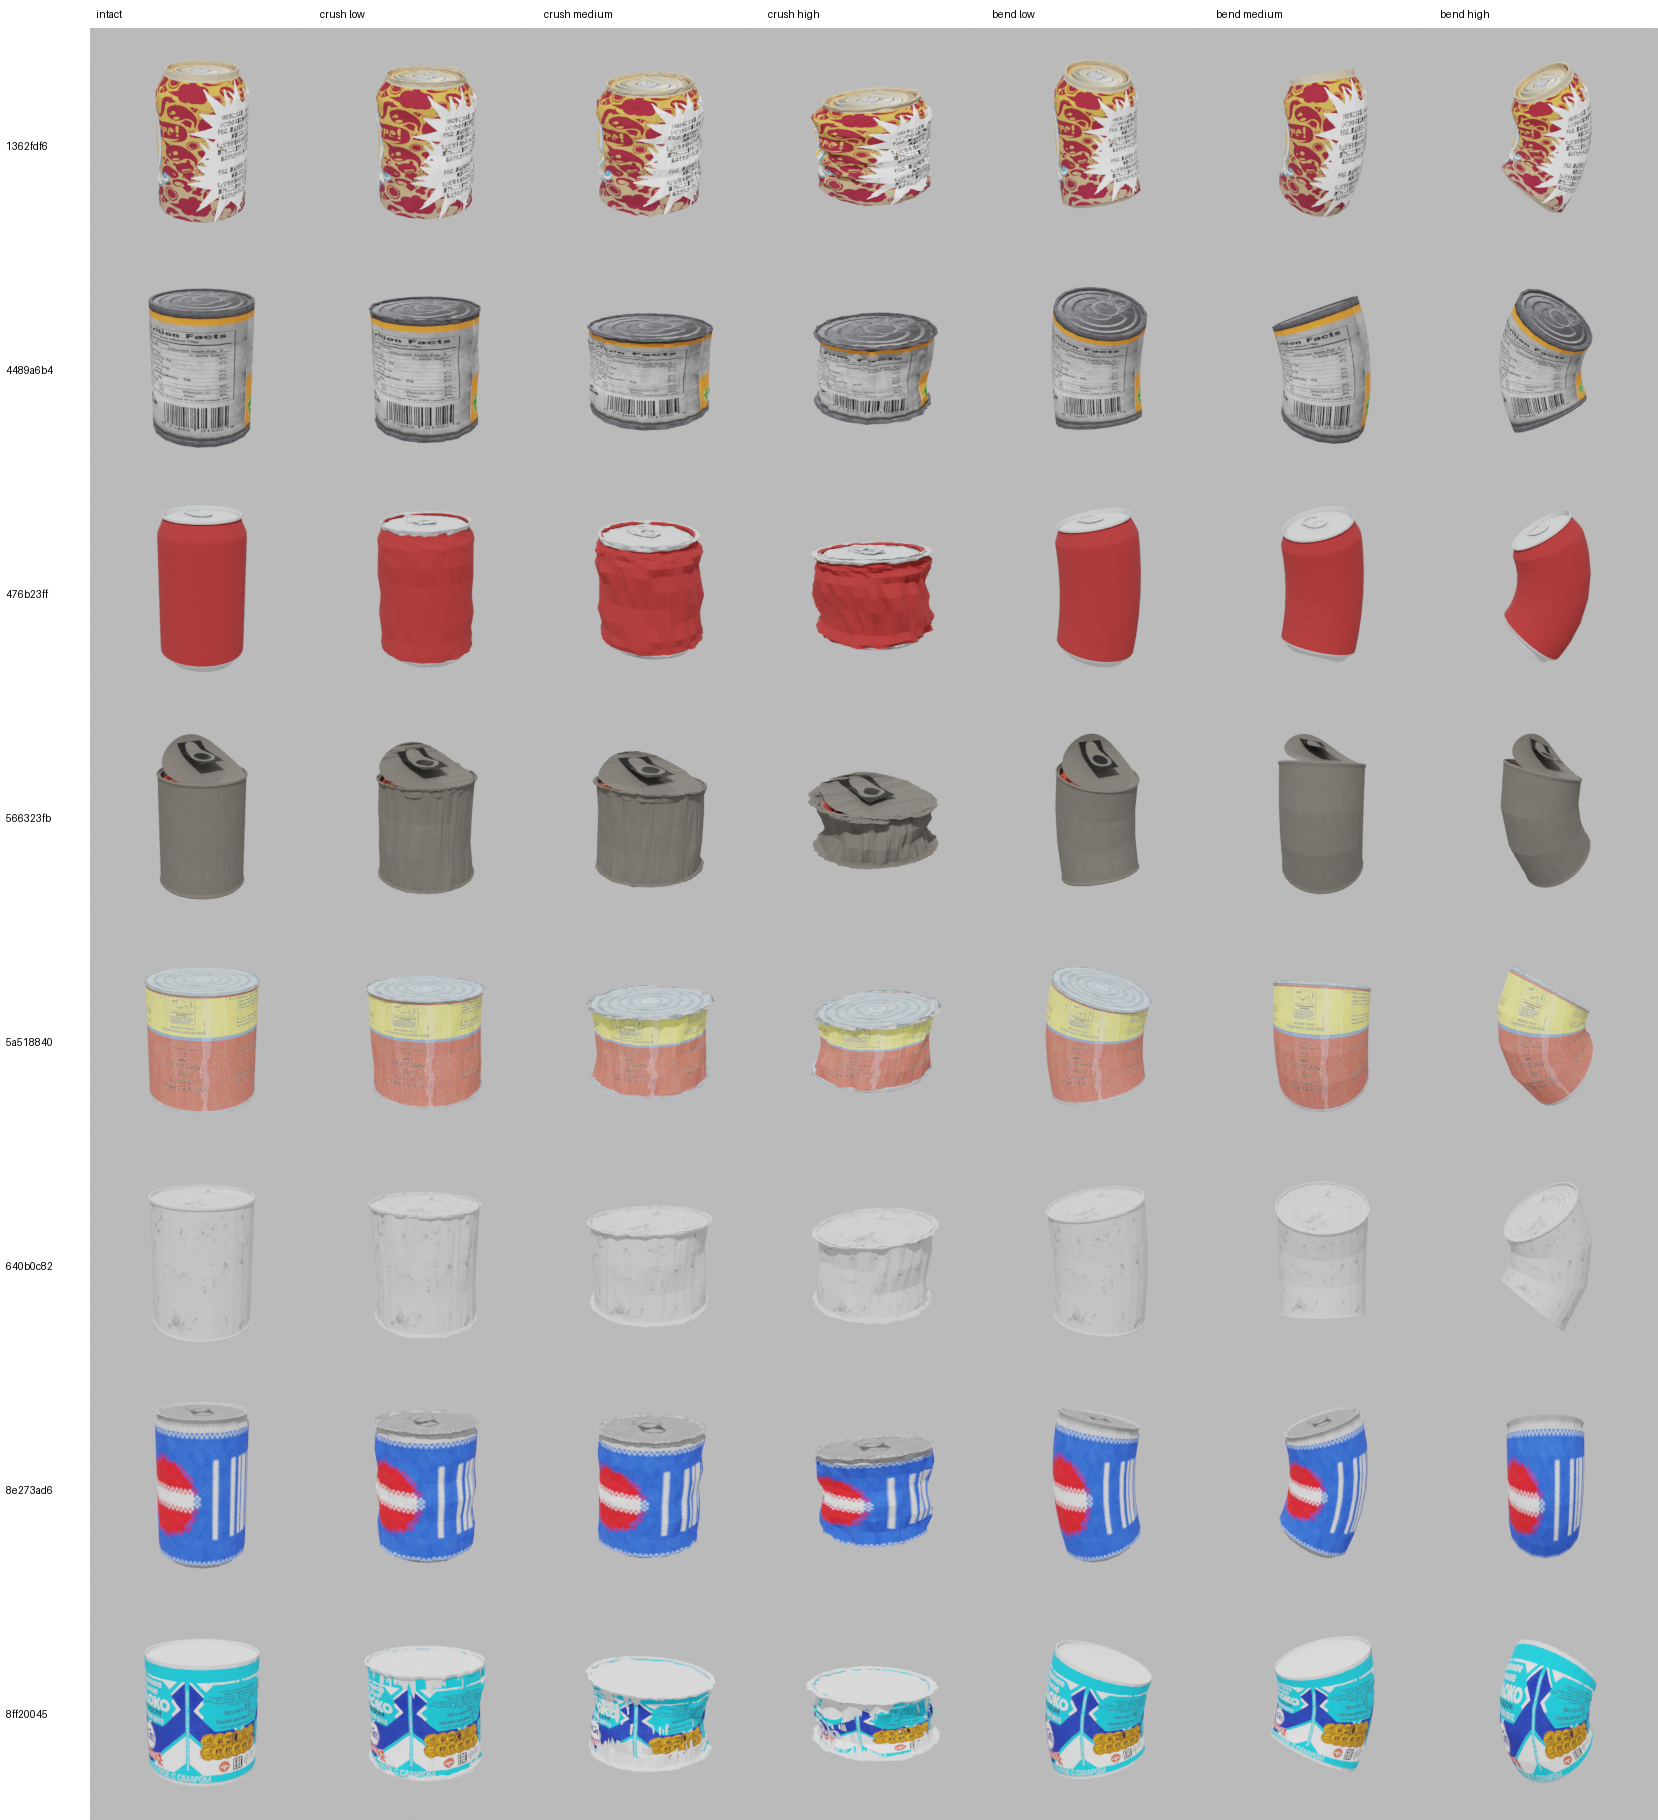
\includegraphics[width=\linewidth]{model_grid_can.png}
  \caption{Cans}
\end{subfigure}\hfill
\begin{subfigure}{0.49\textwidth}
  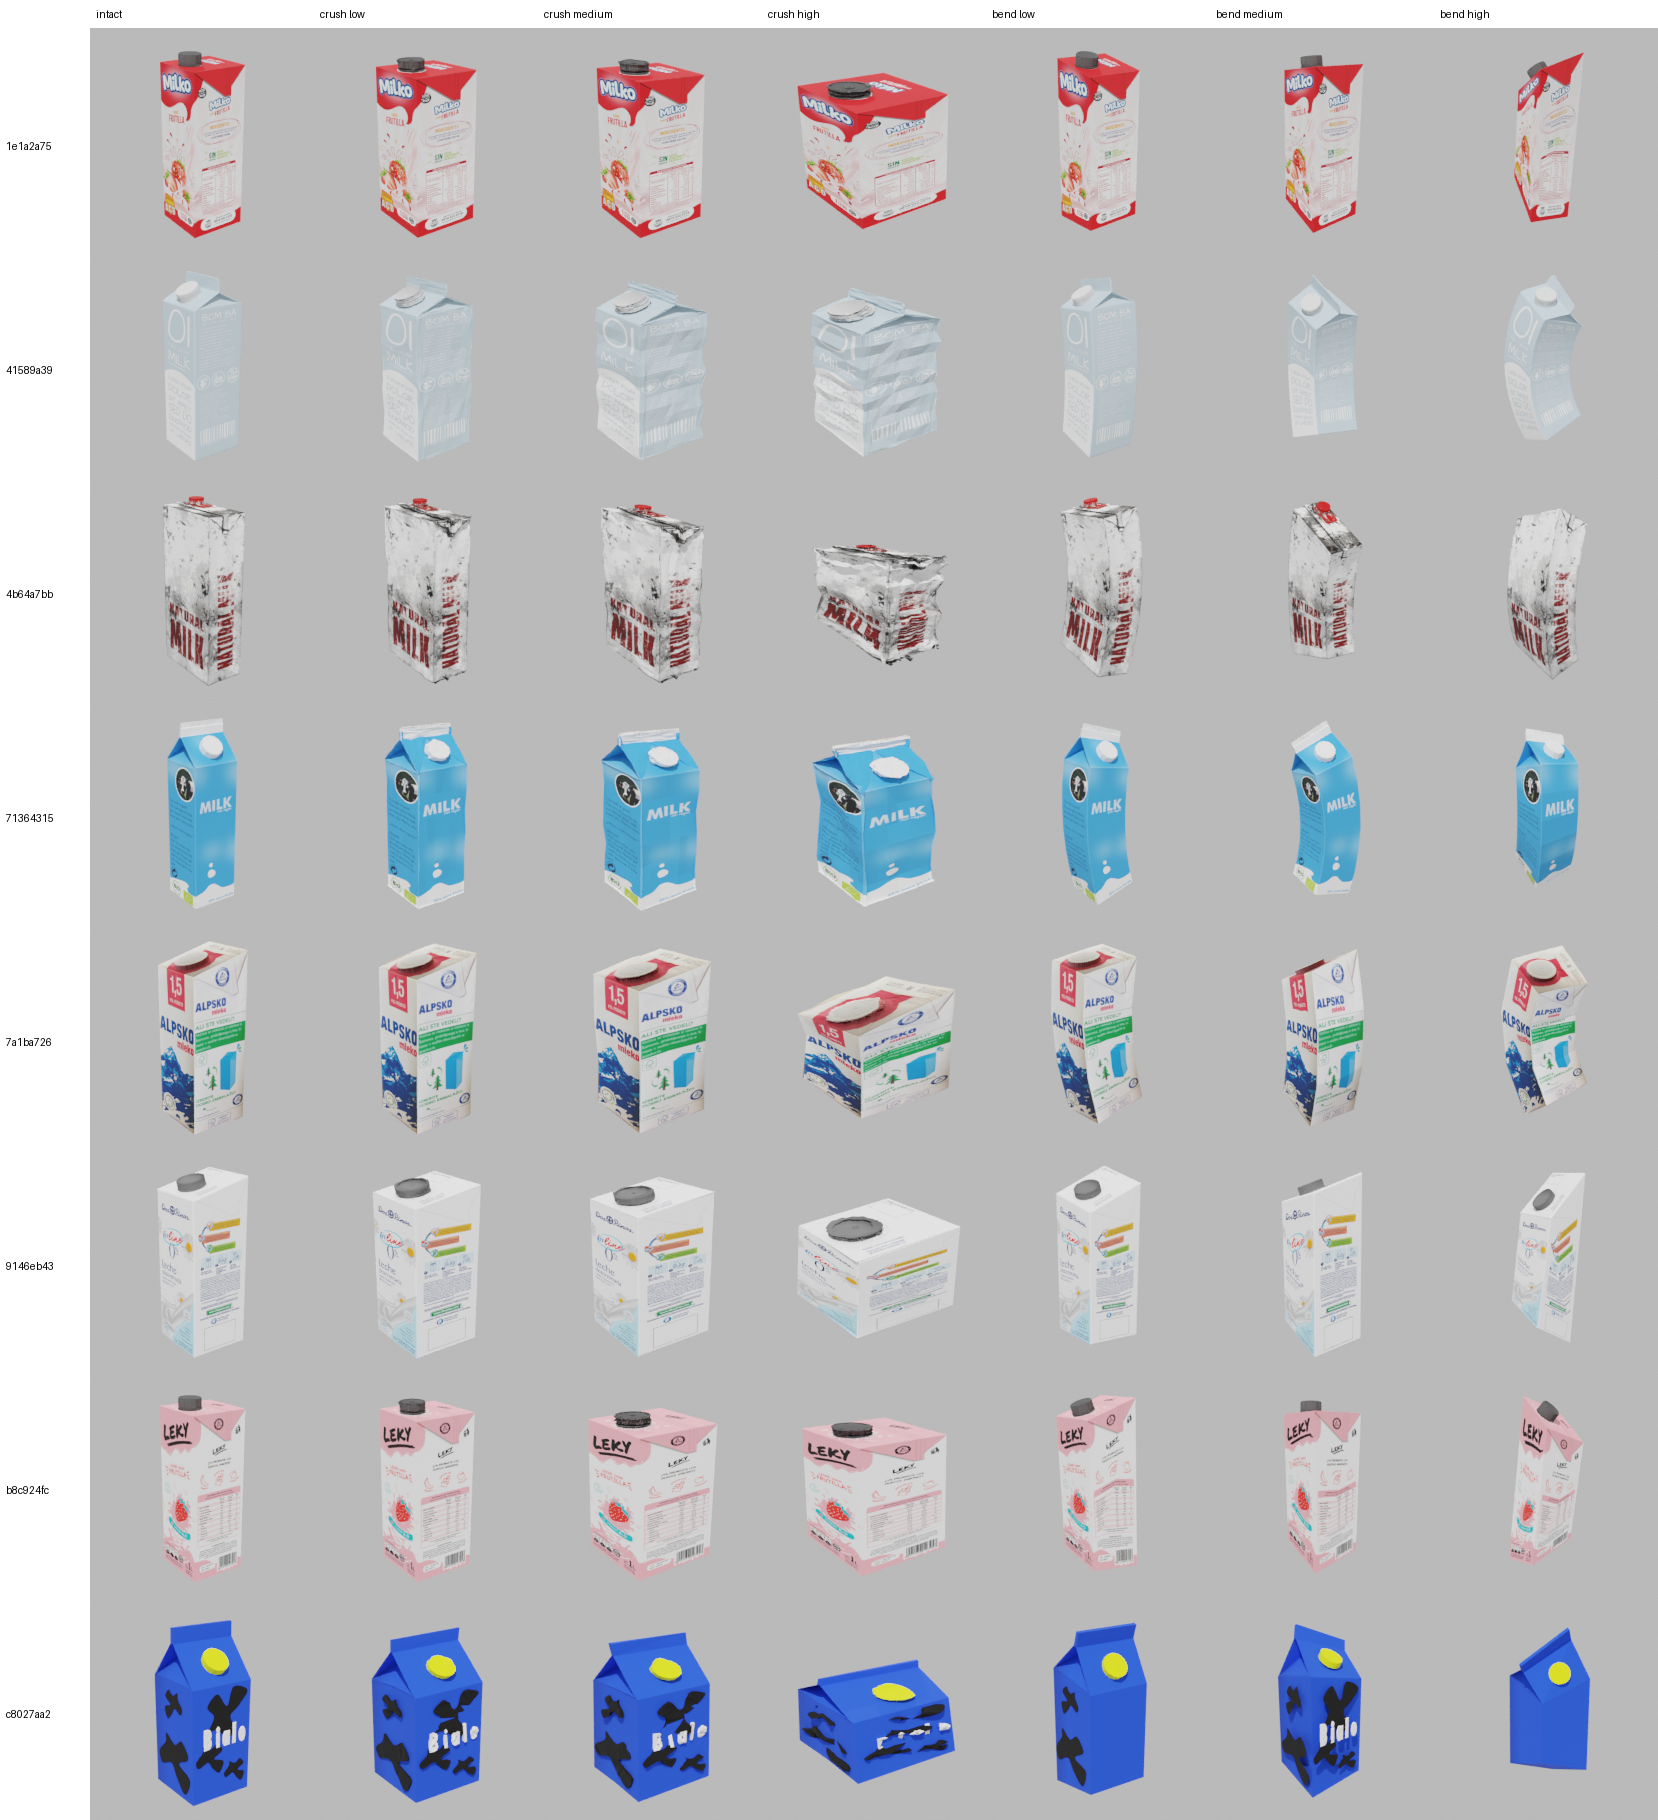
\includegraphics[width=\linewidth]{model_grid_carton.png}
  \caption{Cartons}
\end{subfigure}
\caption{Every source model (rows) intact and at every deformation level (columns: intact,
crush low/medium/high, bend low/medium/high). Grids for bottles and cups are in
\code{outputs/figures/}.}
\label{fig:grids}
\end{figure}

\subsection{Scene generation and automatic annotation}

Scenes are generated with BlenderProc (\code{src/generate\_scenes.py}); Table~\ref{tab:dr}
lists the randomised factors. After placement, all objects are dropped with rigid-body physics so
that they rest naturally, fall over and touch each other. Each scene is rendered from two
camera poses with Cycles at 16 samples and $640\times480$ pixels. Together with the colour image,
BlenderProc renders an instance segmentation map, from which COCO polygon/RLE masks and boxes are
derived; every annotation is linked to its source mesh and receives a \code{deformation} record
(deformed yes/no, type, level, parameters).

\begin{table}[H]
\centering
\small
\begin{tabularx}{\textwidth}{l X}
\toprule
Factor & Randomisation \\
\midrule
Ground & plane with procedural texture (noise, Voronoi, checker, wave), two random colours, random roughness \\
Targets & 1--4 per scene, class and model uniform, intact or deformed with probability $p_\mathrm{def}$ \\
Target materials & roughness 0.1--0.8, metallic 0.3--1.0 for cans and 0--0.2 otherwise, 30\,\% flat random colour \\
Distractors & 0--6 primitives (cube, sphere, cone, monkey), 1.5--6\,cm, random procedural material, unlabelled \\
Lights & 1--3 point lights, 40--300\,W, random position and tint; random ambient strength \\
Camera & 50\,\% top-down (elevation 70--88$^\circ$), 50\,\% oblique (25--60$^\circ$), distance 0.45--0.9\,m, FOV 60$^\circ$ \\
\bottomrule
\end{tabularx}
\caption{Domain randomisation in the scene generator.}
\label{tab:dr}
\end{table}

\begin{figure}[H]
\centering
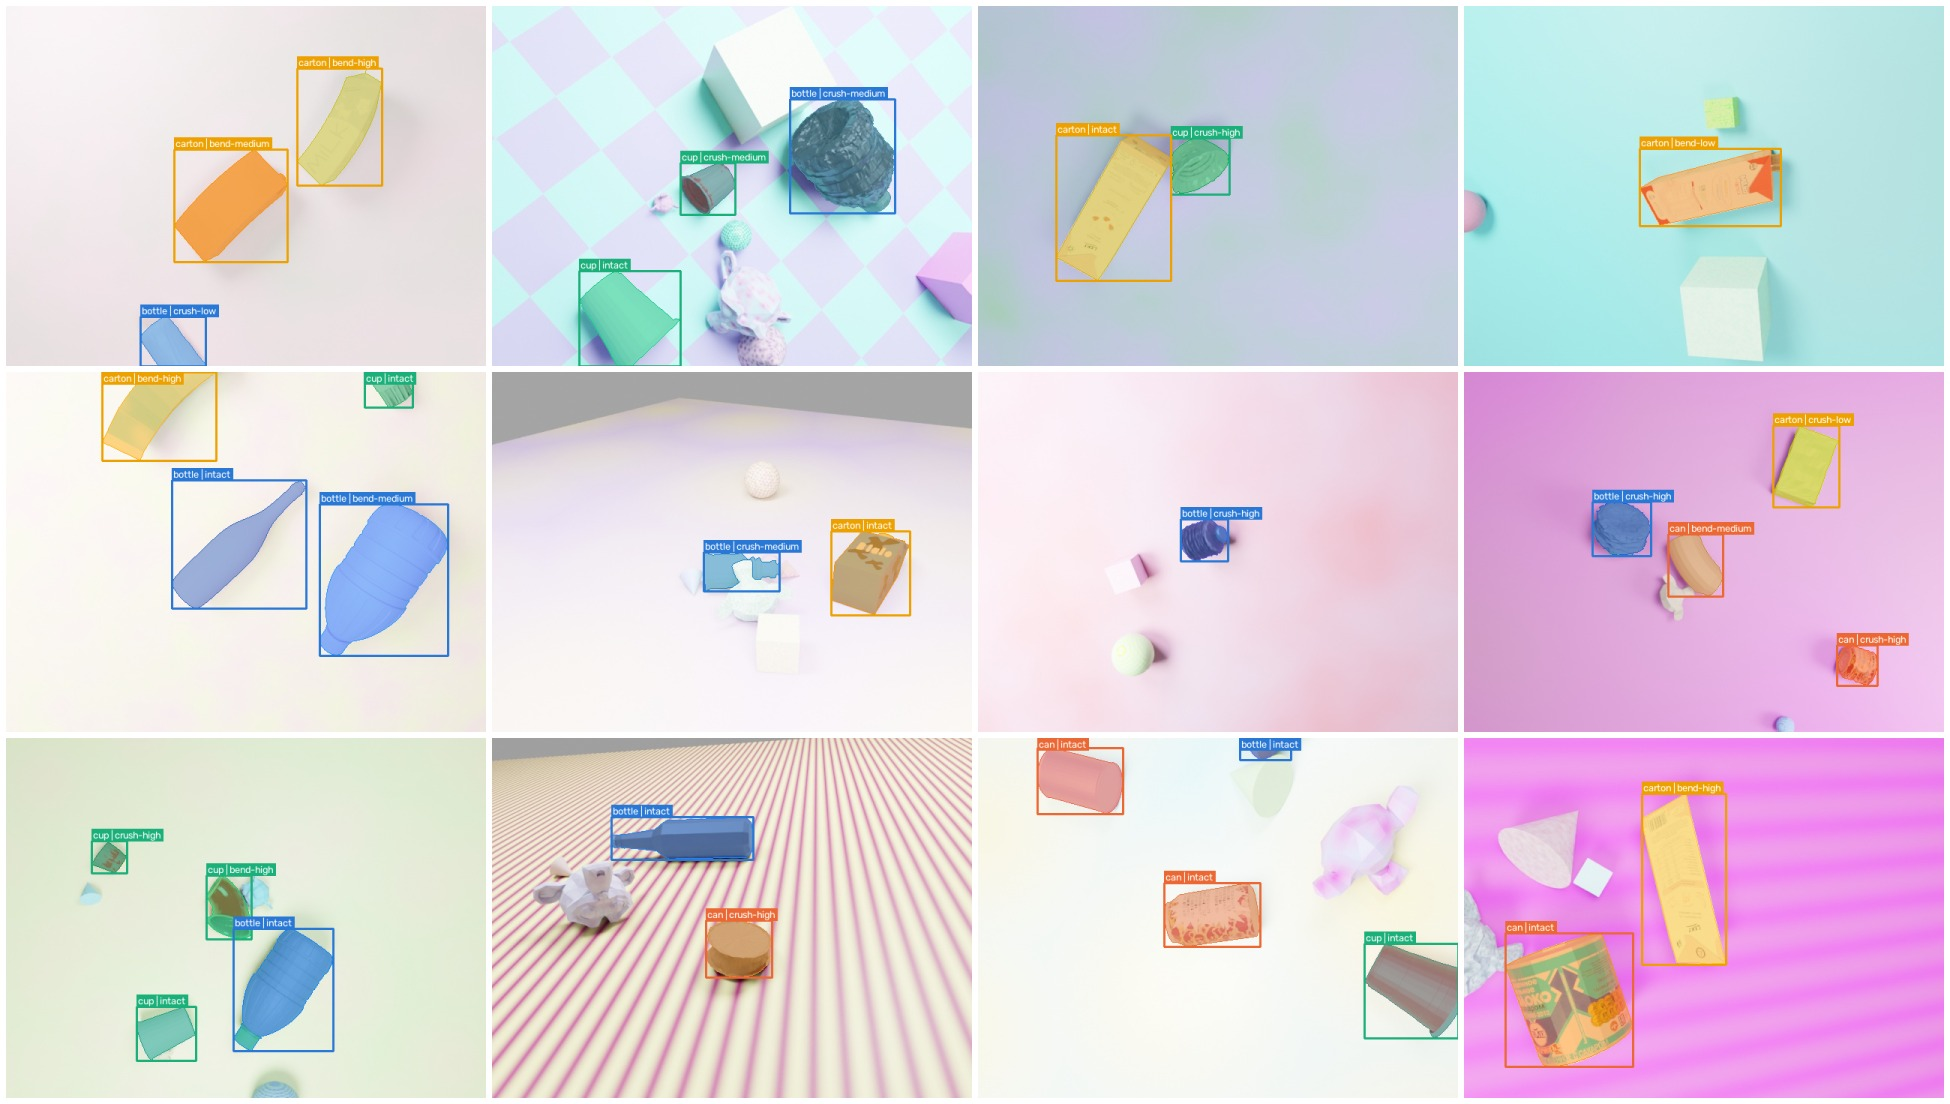
\includegraphics[width=\textwidth]{annotation_grid_B_deformed.jpg}
\caption{Automatically annotated scenes from dataset B: instance masks, bounding boxes and the
label ``class | deformation state''. Distractor primitives are not labelled.}
\label{fig:annot}
\end{figure}

\subsection{Controlled datasets A and B}

Every scene $k$ is generated from its own seed $\mathrm{hash}(\text{seed}, k)$, and the random
draws do not depend on the deformation probability $p_\mathrm{def}$. Rendering with
$p_\mathrm{def}=0.6$ yields \textbf{B\_deformed}; rendering with $p_\mathrm{def}=0$ yields
\textbf{A\_intact}, which contains the same floors, lights, cameras, models and distractors, but
every object that is deformed in B is intact in A (Figure~\ref{fig:design}). Both datasets are
split into train/validation/test sets (80/10/10) \emph{by scene}, so that the two views of a scene
never end up in different splits; the split is identical for A and B.

\begin{figure}[H]
\centering
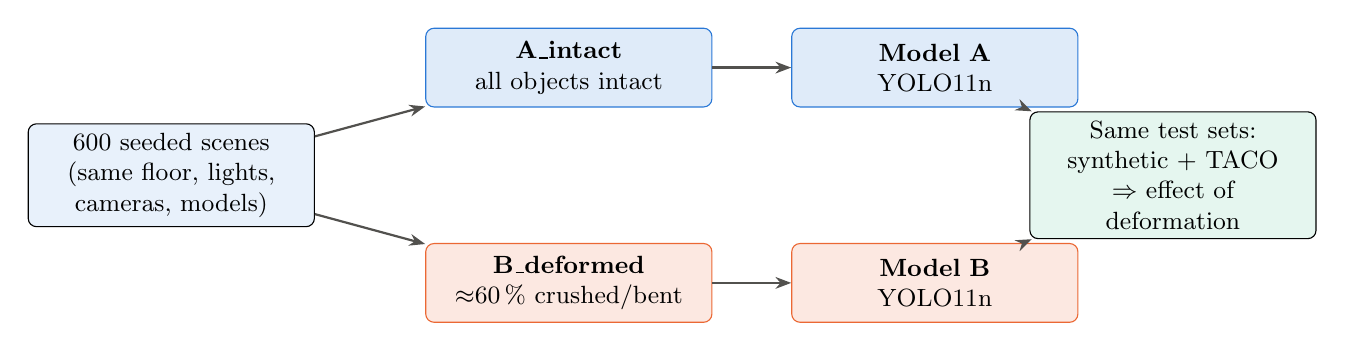
\begin{tikzpicture}[
  every node/.style={font=\small},
  box/.style={draw, rounded corners=3pt, align=center, minimum height=10mm, text width=34mm},
  arr/.style={-{Stealth[length=2mm]}, thick, color=ink2}]
\node[box, fill=stageData] (scene) {600 seeded scenes\\(same floor, lights,\\cameras, models)};
\node[box, fill=seriesA!15, draw=seriesA, above right=2mm and 14mm of scene] (A) {\textbf{A\_intact}\\all objects intact};
\node[box, fill=seriesB!15, draw=seriesB, below right=2mm and 14mm of scene] (B) {\textbf{B\_deformed}\\$\approx$60\,\% crushed/bent};
\node[box, fill=seriesA!15, draw=seriesA, right=10mm of A] (mA) {\textbf{Model A}\\YOLO11n};
\node[box, fill=seriesB!15, draw=seriesB, right=10mm of B] (mB) {\textbf{Model B}\\YOLO11n};
\node[box, fill=stageEval, right=12mm of $(mA)!0.5!(mB)$] (test) {Same test sets:\\synthetic + TACO\\$\Rightarrow$ effect of\\deformation};
\draw[arr] (scene) -- (A); \draw[arr] (scene) -- (B);
\draw[arr] (A) -- (mA); \draw[arr] (B) -- (mB);
\draw[arr] (mA) -- (test); \draw[arr] (mB) -- (test);
\end{tikzpicture}
\caption{Experimental design: identical scenes, the only difference between A and B is object
deformation.}
\label{fig:design}
\end{figure}

\subsection{Real-world test set}

TACO's official annotations and all 1500 images are downloaded; images are stored at 640\,px
(the long side) with their EXIF orientation applied, so that pixels and annotations agree. TACO
categories are mapped onto our four classes (Table~\ref{tab:classes}) and all other litter
categories are dropped. All 1500 images are kept, including those without any of our classes, so
false positives on other litter are counted. TACO is used only for testing.

\subsection{Detector and training}

Both detectors are YOLO11n (Ultralytics~\cite{yolo11}, 2.6\,M parameters), initialised from
COCO-pretrained weights and trained for 60 epochs at 640\,px, batch size 16, with the default
Ultralytics augmentation (mosaic, switched off for the last 10 epochs), on an Apple M2 Pro GPU
(MPS). The two runs use identical hyper-parameters and seed; model selection uses each run's own
validation split.

% ================================================================ results
\section{Experiments and Results}

\subsection{Datasets}

\begin{table}[H]
\centering
\small
\begin{tabular}{l rrr rrr rr}
\toprule
& \multicolumn{3}{c}{B\_deformed} & \multicolumn{3}{c}{A\_intact} & \multicolumn{2}{c}{TACO (real)} \\
\cmidrule(lr){2-4}\cmidrule(lr){5-7}\cmidrule(lr){8-9}
Class & images$^\dagger$ & objects & deformed & images$^\dagger$ & objects & deformed & images$^\dagger$ & objects \\
\midrule
bottle & 593 & 737 & 424 & 592 & 723 & 0 & 322 & 439 \\
can    & 529 & 669 & 392 & 529 & 651 & 0 & 169 & 263 \\
cup    & 556 & 714 & 432 & 535 & 700 & 0 & 158 & 186 \\
carton & 564 & 688 & 427 & 566 & 689 & 0 & 115 & 138 \\
\midrule
total objects & -- & 2808 & 1675 & -- & 2763 & 0 & -- & 1026 \\
\midrule
images in dataset & \multicolumn{3}{c}{1200 (all contain $\ge$1 object)} & \multicolumn{3}{c}{1200 (all contain $\ge$1 object)} & \multicolumn{2}{c}{1500 (658 with $\ge$1 object)} \\
\bottomrule
\end{tabular}
\caption{Dataset statistics. $^\dagger$``images'' = number of images in which the class appears
at least once. Most images contain several classes (2.3 objects per image on average), so this
column does \emph{not} add up to the number of images; the bottom row gives the actual number of
images. Small differences between A and B come from objects whose visibility changes when their
shape changes.}
\label{tab:data}
\end{table}

Each class appears in 529--593 of the 1200 images of each synthetic dataset, and the deformed
objects in B are spread evenly over the six type/level combinations (54--85 objects per class and
combination).

\subsection{Training}

\begin{figure}[H]
\centering
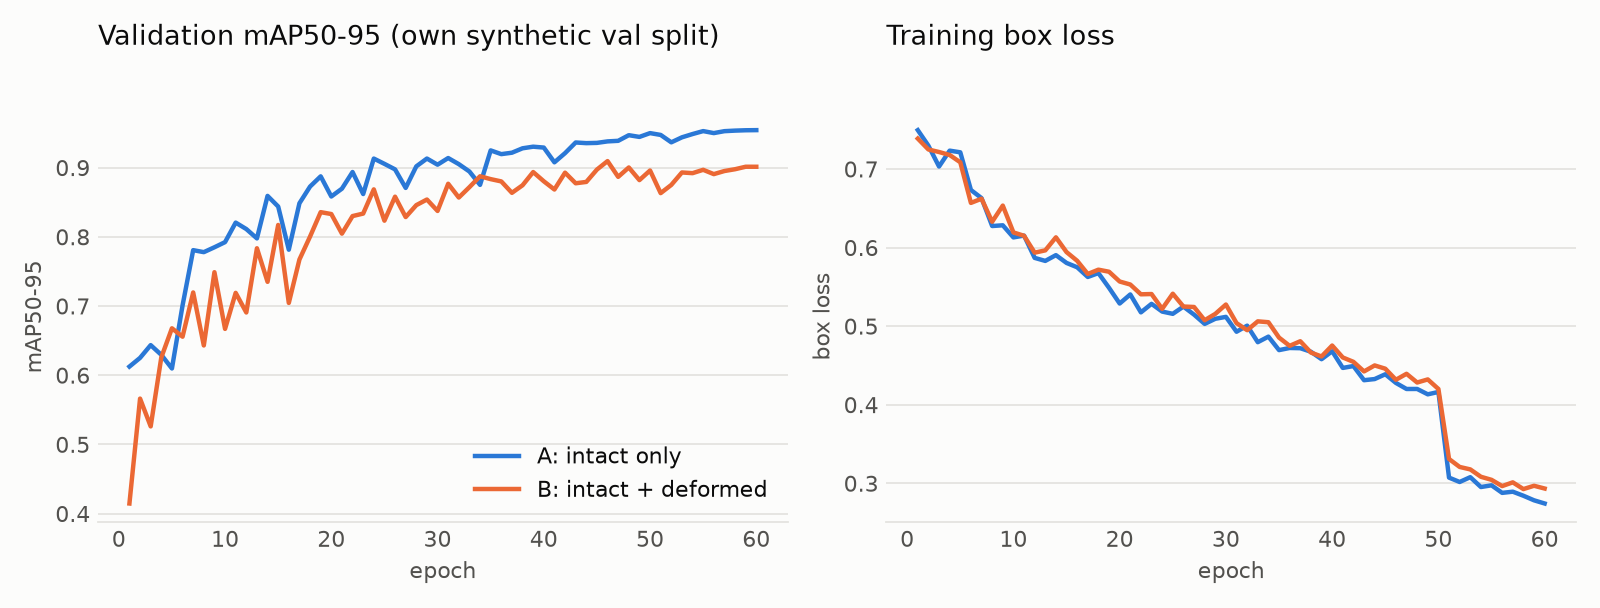
\includegraphics[width=\textwidth]{results_training_curves.png}
\caption{Training of models A and B. Left: mAP50-95 on each model's own synthetic validation
split (B's split contains deformed objects and is therefore harder). Right: training box loss;
the step at epoch 50 is where mosaic augmentation is switched off.}
\label{fig:curves}
\end{figure}

Training took 31 minutes (A) and 45 minutes (B, partly in parallel with rendering). Both models
converge smoothly; their final validation mAP50-95 is 0.954 (A) and 0.901 (B).

\subsection{Overall detection accuracy}

\begin{table}[H]
\centering
\small
\begin{tabular}{l l cccc}
\toprule
Test set & Model & Precision & Recall & mAP50 & mAP50-95 \\
\midrule
\multirow{2}{*}{Synthetic, deformed objects (120 imgs)} & A & 0.909 & 0.810 & 0.889 & 0.868 \\
 & B & 0.910 & \textbf{0.871} & \textbf{0.936} & \textbf{0.914} \\
\midrule
\multirow{2}{*}{Synthetic, intact objects (120 imgs)} & A & \textbf{0.964} & 0.881 & \textbf{0.965} & \textbf{0.937} \\
 & B & 0.933 & \textbf{0.898} & 0.953 & 0.919 \\
\midrule
\multirow{2}{*}{Real TACO photos (1500 imgs)} & A & \textbf{0.156} & 0.112 & 0.042 & 0.033 \\
 & B & 0.137 & \textbf{0.137} & \textbf{0.051} & \textbf{0.037} \\
\bottomrule
\end{tabular}
\caption{Overall results of model A (trained on intact objects) and model B (trained with
deformed objects) on the three test sets.}
\label{tab:overall}
\end{table}

\begin{figure}[H]
\centering
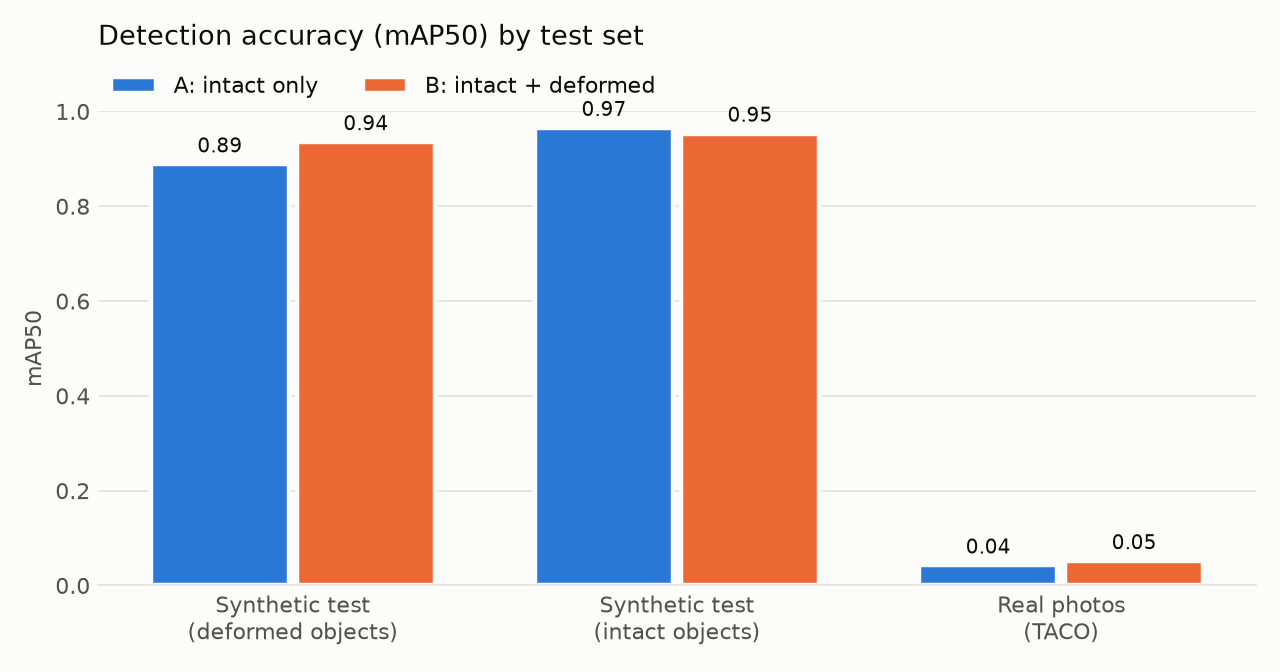
\includegraphics[width=0.85\textwidth]{results_map50.png}
\caption{mAP50 of models A and B on the three test sets.}
\label{fig:map}
\end{figure}

\subsection{Effect of deformation type and level}

To understand where the difference comes from, predictions on the deformed synthetic test scenes
are matched to the ground truth (same class, IoU $\ge 0.5$, confidence $\ge 0.25$) and recall is
computed per deformation type and level (Table~\ref{tab:recall}, Figure~\ref{fig:recall}).

\begin{table}[H]
\centering
\small
\begin{tabular}{l c ccc ccc}
\toprule
& & \multicolumn{3}{c}{crush} & \multicolumn{3}{c}{bend} \\
\cmidrule(lr){3-5}\cmidrule(lr){6-8}
Model & intact & low & medium & high & low & medium & high \\
\midrule
A & 0.93 & 0.90 & 0.66 & 0.45 & 0.96 & \textbf{0.92} & \textbf{0.93} \\
B & \textbf{0.94} & \textbf{0.97} & \textbf{0.93} & \textbf{0.52} & \textbf{1.00} & 0.88 & 0.91 \\
\midrule
objects & 111 & 29 & 29 & 31 & 26 & 25 & 43 \\
\bottomrule
\end{tabular}
\caption{Recall by deformation on the synthetic test scenes (all classes).}
\label{tab:recall}
\end{table}

\begin{figure}[H]
\centering
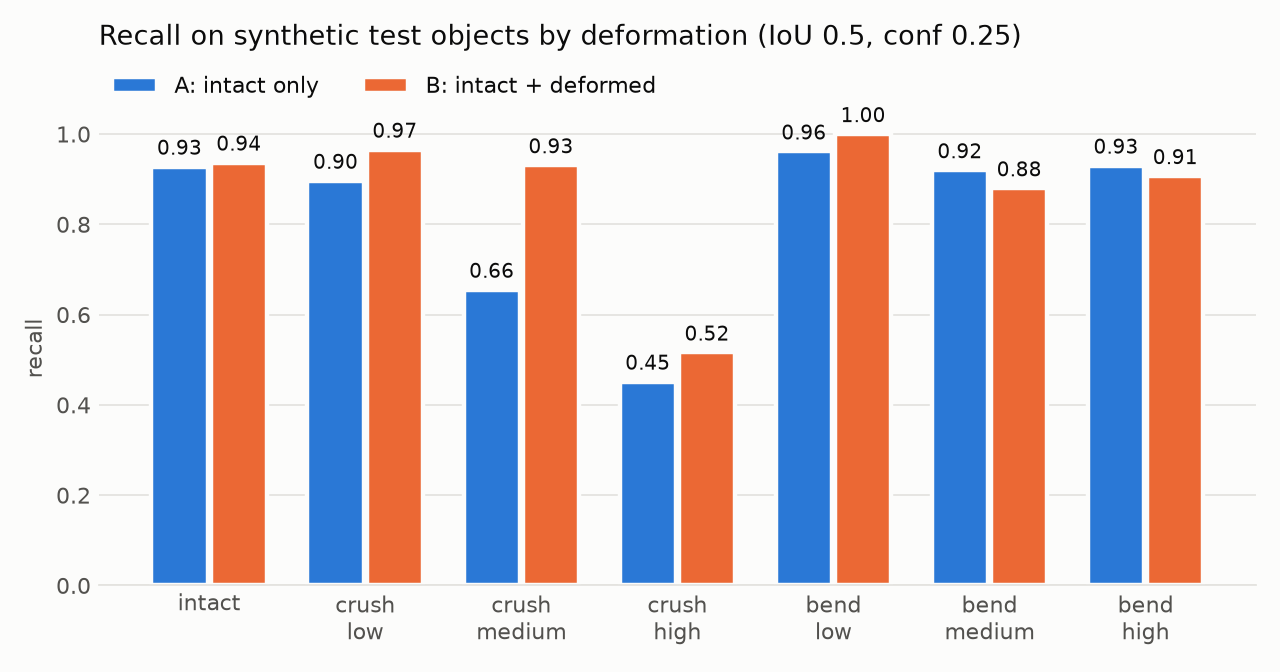
\includegraphics[width=0.85\textwidth]{results_recall_deformation.png}
\caption{Recall by deformation type and level on the synthetic test scenes.}
\label{fig:recall}
\end{figure}

\subsection{Real-world (sim-to-real) results per class}

\begin{table}[H]
\centering
\small
\begin{tabular}{l c cc cc}
\toprule
& & \multicolumn{2}{c}{AP50} & \multicolumn{2}{c}{Recall} \\
\cmidrule(lr){3-4}\cmidrule(lr){5-6}
Class & TACO objects & A & B & A & B \\
\midrule
bottle & 439 & 0.017 & \textbf{0.032} & 0.041 & \textbf{0.091} \\
can    & 263 & 0.068 & \textbf{0.072} & 0.213 & \textbf{0.243} \\
cup    & 186 & 0.057 & \textbf{0.068} & 0.070 & \textbf{0.075} \\
carton & 138 & 0.026 & \textbf{0.034} & 0.123 & \textbf{0.138} \\
\bottomrule
\end{tabular}
\caption{Per-class results on real TACO photos.}
\label{tab:taco}
\end{table}

\begin{figure}[H]
\centering
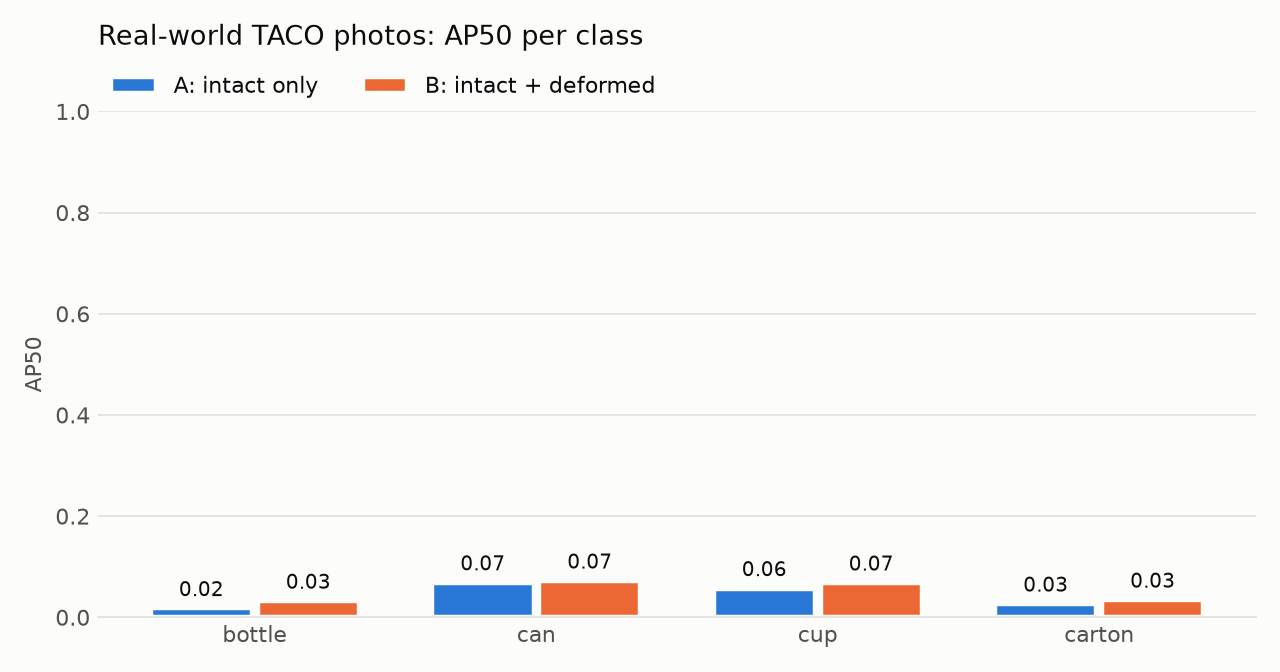
\includegraphics[width=0.85\textwidth]{results_taco_per_class.png}
\caption{AP50 per class on real TACO photos.}
\label{fig:taco}
\end{figure}

\begin{figure}[H]
\centering
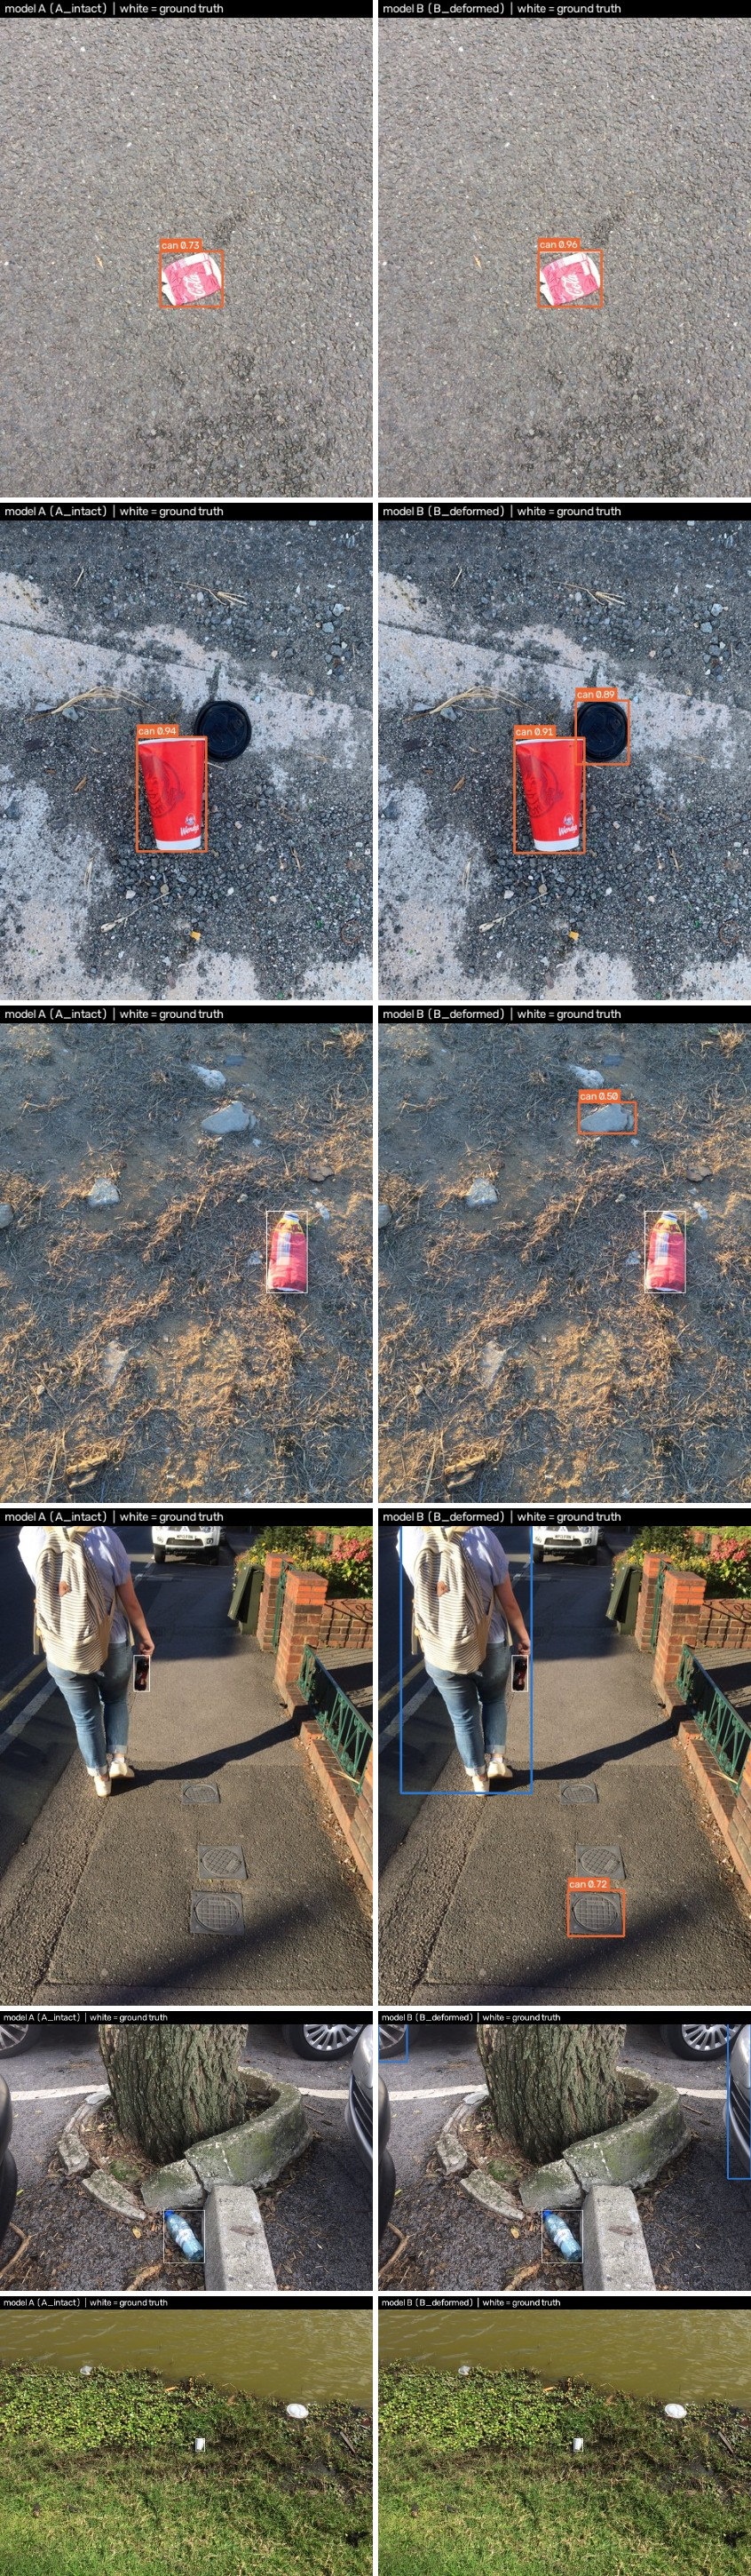
\includegraphics[height=0.82\textheight]{predictions_taco.jpg}
\caption{Predictions of model A (left) and model B (right) on the same TACO photos (white boxes:
ground truth; coloured boxes: predictions with confidence $\ge 0.4$). Typical behaviour: both
models detect clearly visible items on plain ground; errors include confusing a cup with a can,
false positives on round street objects, and missed small or occluded items.}
\label{fig:pred}
\end{figure}

\begin{figure}[H]
\centering
\includegraphics[width=0.6\textwidth]{B_deformed_on_taco/confusion_matrix_normalized.png}
\caption{Normalised confusion matrix of model B on TACO. Most errors are missed objects
(predicted as background) rather than confusions between the four classes.}
\label{fig:cm}
\end{figure}

% ================================================================ discussion
\section{Discussion}

\paragraph{Deformation matters for detection, mainly crushing.} The detector trained only on
intact models generalises well to bent objects (recall 0.92--0.96), but loses a third of
medium-crushed and more than half of heavily crushed objects. Training on deformed objects
recovers most of the medium-crushed objects (0.66 $\rightarrow$ 0.93) and improves mAP50 on
deformed scenes by 4.7 points, while costing only 1.2 points on intact objects. Heavily crushed
objects remain hard for both models (0.45 vs.\ 0.52), since they lose most of their
characteristic silhouette.

\paragraph{Sim-to-real.} On real photos, model B outperforms model A overall (mAP50 +0.009,
i.e.\ +22\,\% relative; recall 0.112 $\rightarrow$ 0.137) and on all four classes, which is
consistent with our hypothesis. However, absolute performance is very low for both models
(mAP50 $\approx 0.05$). The appearance gap between our renders and real litter photos clearly
dominates: our scenes have clean procedural floors, no dirt, grass, gravel or clutter, perfect
labels and only eight shape/texture prototypes per class, whereas TACO objects are dirty, torn,
partly buried, often small and photographed in complex natural scenes. The improvement on TACO
comes from a single training run per model and is small in absolute terms; it is therefore an
encouraging indication rather than a statistically established effect.

\paragraph{Limitations.}
\begin{itemize}
  \item Only 8 source models per class, as Objaverse contains few clean, CC-licensed cups and
        cartons.
  \item Deformation is geometric (modifiers), not a physical simulation; glass bottles are
        crushed like plastic and a few models show inner surfaces at high crush levels.
  \item TACO has no deformation labels, so the per-level analysis is only possible on synthetic
        data; TACO's ``Other carton'' also contains non-drink cardboard, and cup and carton test
        counts are small.
  \item One training run per model, small detector (YOLO11n) and 60 epochs on a laptop GPU.
\end{itemize}

% ================================================================ conclusion
\section{Conclusion and Future Work}

We built a reproducible, configurable pipeline that turns intact Objaverse models into a
labelled synthetic dataset of deformable waste, and used two matched datasets to measure the
effect of deformation on object detection. Procedural deformation substantially improves the
detection of crushed objects in synthetic scenes without hurting intact objects, and gives a
small, consistent improvement on real litter photos across all classes. The dominant remaining
obstacle is the appearance gap between renders and real photographs.

Future work, in order of expected impact:
\begin{enumerate}
  \item realistic backgrounds (photo or HDRI textures of asphalt, grass, sand, gravel) and
        natural clutter;
  \item dirt, wear and torn-label textures, and physically simulated deformation;
  \item more source models per class and additional classes (plastic bags, wrappers);
  \item fine-tuning with a small amount of real data, and multiple training seeds to establish
        statistical significance;
  \item larger detectors and longer training.
\end{enumerate}

% ================================================================ references
\begin{thebibliography}{9}
\bibitem{objaverse} M.~Deitke et al., ``Objaverse: A Universe of Annotated 3D Objects,'' in
  \emph{Proc.\ CVPR}, 2023.
\bibitem{blenderproc} M.~Denninger et al., ``BlenderProc2: A Procedural Pipeline for
  Photorealistic Rendering,'' \emph{Journal of Open Source Software}, 8(82), 2023.
\bibitem{taco} P.~F.~Proen\c{c}a and P.~Sim\~{o}es, ``TACO: Trash Annotations in Context for
  Litter Detection,'' arXiv:2003.06975, 2020.
\bibitem{tobin} J.~Tobin et al., ``Domain Randomization for Transferring Deep Neural Networks
  from Simulation to the Real World,'' in \emph{Proc.\ IROS}, 2017.
\bibitem{tremblay} J.~Tremblay et al., ``Training Deep Networks with Synthetic Data: Bridging the
  Reality Gap by Domain Randomization,'' in \emph{Proc.\ CVPR Workshops}, 2018.
\bibitem{yolo11} G.~Jocher, J.~Qiu, ``Ultralytics YOLO11,'' 2024.
  \url{https://github.com/ultralytics/ultralytics}
\end{thebibliography}

% ================================================================ appendix
\appendix
\section{Repository Structure}

\begin{lstlisting}
AI-Project/
|-- README.md                 overview, how to run, results
|-- requirements.txt          Python dependencies (.venv, Python 3.11)
|-- run_pipeline.py           runs all stages in order (one command)
|-- run_blenderproc.sh        runs Blender scripts with the local Blender copy
|-- configs/pipeline.yaml     classes, sizes, deformation ranges, dataset size, training
|-- docs/                     plan.md, references.md
|-- report/                   this report (report.tex, report.pdf)
|-- src/
|   |-- config.py               loads the config, project paths
|   |-- mesh_utils.py           mesh loading, class-specific shape checks
|   |-- download_objaverse.py   stage 1: fetch models
|   |-- normalize.py            stage 2: upright, real size, OBJ
|   |-- deform.py               stage 3: crush / bend (Blender)
|   |-- render_model_grid.py    figure: models x deformation levels (Blender)
|   |-- generate_scenes.py      stage 4: scenes + COCO annotations (BlenderProc)
|   |-- coco_to_yolo.py         stage 5: YOLO labels, scene-level split
|   |-- visualize_annotations.py  overlays and statistics
|   |-- prepare_taco.py         real test set
|   |-- train_yolo.py           stage 6: YOLO11n training
|   |-- evaluate.py             stage 7: metrics, recall by deformation, examples
|   `-- make_report.py          stage 8: charts and results tables
|-- assets/models/
|   |-- raw/<class>/            original Objaverse GLB files
|   |-- normalized/<class>/     clean OBJ models
|   |-- deformed/<class>/<id>/  <type>_<level>_<k>.obj/.mtl/.json
|   `-- LICENSES.csv            model credits and licences
|-- data/
|   |-- synthetic/A_intact/     coco_data/, yolo/, instance_metadata.csv, scene_metadata.jsonl
|   |-- synthetic/B_deformed/   same structure
|   |-- synthetic/pilot_50/     earlier 2-class pilot (archived)
|   `-- real/taco/              TACO images + COCO + YOLO (test only)
|-- train/runs/<run>/          training curves, confusion matrices, weights
|-- train/weights/             A_intact.pt, B_deformed.pt
|-- outputs/figures/           all figures used in this report
|-- outputs/results/           metrics CSVs, results.md, validation plots
`-- logs/                      one log per pipeline stage
\end{lstlisting}

\section{Reproducing the Results}

\begin{lstlisting}
cd ~/Desktop/AI-Project
python3.11 -m venv .venv && .venv/bin/pip install -r requirements.txt
.venv/bin/python run_pipeline.py --stages all      # complete pipeline (~3-4 h on an M2 Pro)
.venv/bin/python run_pipeline.py --from train      # only training, evaluation and report
.venv/bin/python run_pipeline.py --stages all --dry-run   # list the commands
\end{lstlisting}

All parameters are set in \code{configs/pipeline.yaml}; each stage writes a log to
\code{logs/<stage>.log}. The report itself is compiled with
\code{cd report \&\& latexmk -pdf report.tex}.

\end{document}
